\usetikzlibrary{shapes,backgrounds}

\def \setA{ (0,0) circle (.75cm) }
\def \setB{ (60:.75) circle (.75cm) }
\def \setC{ (.75,0) circle (.75cm) }



\begin{enumerate}\setcounter{enumii}{2}
  \item $A \cap (B \cup C) = (A \cap B) \cup (A \cap C)$ \\

\begin{minipage}{.23\textwidth}

  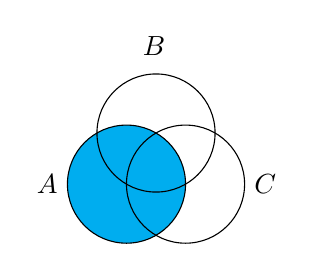
\begin{tikzpicture}

    \begin{scope}
      \fill[cyan] \setA;
    \end{scope}

    \draw \setA;
    \draw \setB;
    \draw \setC;
    \draw (-.75,0) node[left] {$A$};
    \draw (.35,1.75) node {$B$};
    \draw (1.5,0) node[right] {$C$};

  \end{tikzpicture}

\end{minipage}
$\cap$
\begin{minipage}{.23\textwidth}

  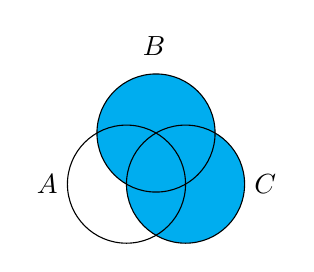
\begin{tikzpicture}

    \begin{scope}
      \fill[cyan] \setB;
      \fill[cyan] \setC;
    \end{scope}

    \draw \setA;
    \draw \setB;
    \draw \setC;
    \draw (-.75,0) node[left] {$A$};
    \draw (.35,1.75) node {$B$};
    \draw (1.5,0) node[right] {$C$};

  \end{tikzpicture}

\end{minipage}
=
\begin{minipage}{.23\textwidth}

  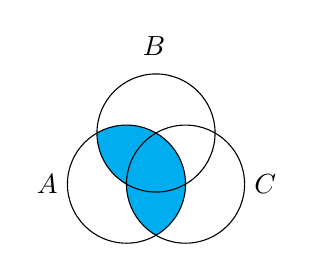
\begin{tikzpicture}

    \begin{scope}
      \clip \setA;
      \fill[cyan] \setB;
    \end{scope}

    \begin{scope}
      \clip \setC;
      \fill[cyan] \setA;
    \end{scope}

    \draw \setA;
    \draw \setB;
    \draw \setC;
    \draw (-.75,0) node[left] {$A$};
    \draw (.35,1.75) node {$B$};
    \draw (1.5,0) node[right] {$C$};

  \end{tikzpicture}

\end{minipage} \\ \\ \\
$\null \qquad\quad\ \ A \qquad\qquad\  \cap \ \ \qquad(B \cup C)$
 \\ \\ \\

\begin{minipage}{.23\textwidth}

  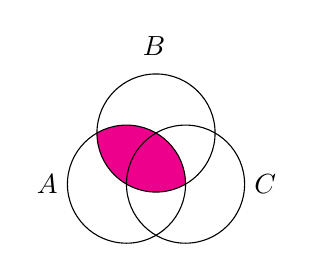
\begin{tikzpicture}

    \begin{scope}
      \clip \setA;
      \fill[magenta] \setB;
    \end{scope}

    \draw \setA;
    \draw \setB;
    \draw \setC;
    \draw (-.75,0) node[left] {$A$};
    \draw (.35,1.75) node {$B$};
    \draw (1.5,0) node[right] {$C$};

  \end{tikzpicture}

\end{minipage}
$\cup$
\begin{minipage}{.23\textwidth}

  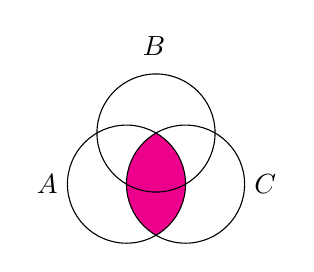
\begin{tikzpicture}

    \begin{scope}
      \clip \setA;
      \fill[magenta] \setC;
    \end{scope}

    \draw \setA;
    \draw \setB;
    \draw \setC;
    \draw (-.75,0) node[left] {$A$};
    \draw (.35,1.75) node {$B$};
    \draw (1.5,0) node[right] {$C$};

  \end{tikzpicture}

\end{minipage}
=
\begin{minipage}{.23\textwidth}

  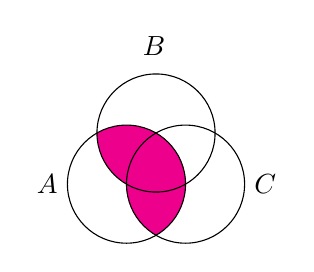
\begin{tikzpicture}

    \begin{scope}
      \clip \setA;
      \fill[magenta] \setC;
    \end{scope}

    \begin{scope}
      \clip \setA;
      \fill[magenta] \setB;
    \end{scope}

    \draw \setA;
    \draw \setB;
    \draw \setC;
    \draw (-.75,0) node[left] {$A$};
    \draw (.35,1.75) node {$B$};
    \draw (1.5,0) node[right] {$C$};

  \end{tikzpicture}

\end{minipage}  \\ \\ \\
$\null \qquad\ (A \cap B) \qquad\ \  \cup \ \ \qquad(A \cup C)$ \\

\end{enumerate}
